\documentclass[11pt]{article}
\usepackage[a4paper,margin=1in]{geometry}
\usepackage{amsmath,amssymb,amsthm}
\usepackage{graphicx}
\usepackage[hidelinks]{hyperref}

\newtheorem{theorem}{Theorem}
\newtheorem{corollary}{Corollary}
\newtheorem{remark}{Remark}

\DeclareMathOperator{\Lip}{Lip}
\DeclareMathOperator{\Ext}{Ext}

\title{Bidual-Complemented Codomains and the Extendable Quotient Model for \(\Lip_0(X,Y)/L(X,Y)\)}
\author{Automatic math-discovery packet}
\date{June 29, 2026}

\begin{document}
\maketitle

\section*{Source questions}

The source paper is Anil Kumar Karn and Arindam Mandal,
\emph{Position of \(L(X,Y)\) in \(\Lip_0(X,Y)\)}, arXiv:2506.09324.
It records the following two questions.

\begin{figure}[h]
\centering

\includegraphics[width=0.93\textwidth]{figures/open_problem_crop.png}
\caption{Question 1.1 asks whether \(L(X,Y)\) is complemented in \(\Lip_0(X,Y)\).}
\end{figure}

\begin{figure}[h]
\centering
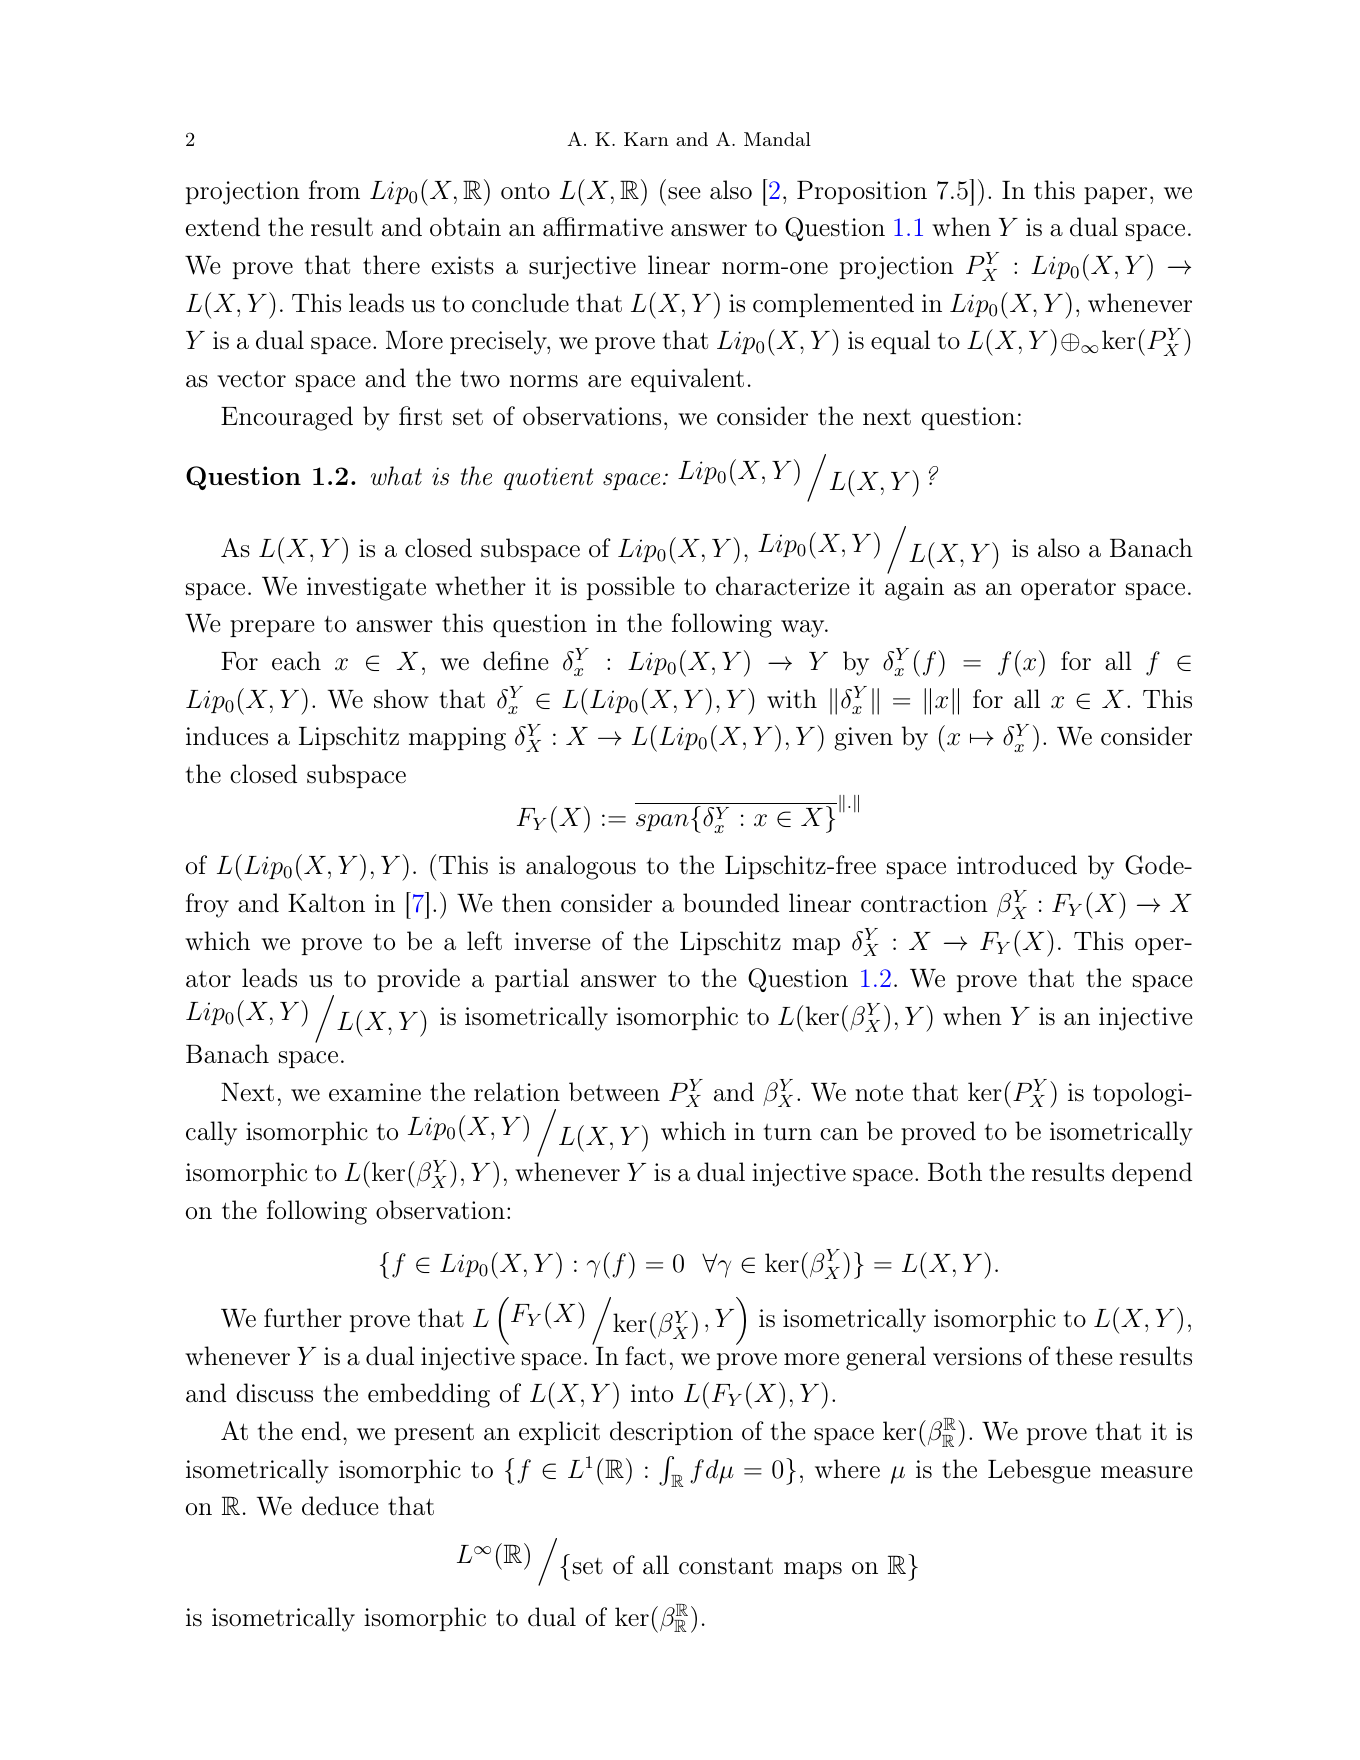
\includegraphics[width=0.93\textwidth]{figures/quotient_question_crop.png}
\caption{Question 1.2 asks for the quotient \(\Lip_0(X,Y)/L(X,Y)\). The source proves the usual operator-space description when \(Y\) is injective.}
\end{figure}

\clearpage

\section*{Source inputs}

We use the following results and notation from Karn--Mandal.

\begin{enumerate}
\item If \(Z\) is a dual Banach space, then there is a norm-one projection
\[
  P_X^Z:\Lip_0(X,Z)\longrightarrow L(X,Z).
\]
\item The vector-valued Lipschitz-free space \(F_Y(X)\), the map
\(\delta_X^Y:X\to F_Y(X)\), and the contraction
\(\beta_X^Y:F_Y(X)\to X\) are defined in the source paper.
\item The map
\[
  \Delta_X^Y:L(F_Y(X),Y)\longrightarrow \Lip_0(X,Y),
  \qquad \Delta_X^Y(A)=A\circ \delta_X^Y,
\]
is a surjective linear isometry.
\item With \(D=\ker(\beta_X^Y)\), the source paper proves
\[
  L(X,Y)={}^{\diamondsuit}D
  :=\{f\in \Lip_0(X,Y):\gamma(f)=0\ \hbox{for all }\gamma\in D\}.
\]
\end{enumerate}

\section*{Proof intuition}

The dual-codomain projection of Karn--Mandal can be used one level above
the desired codomain. If \(Y\) sits complemented inside a dual space \(Z\),
send a \(Y\)-valued Lipschitz map into \(Z\), project it to a \(Z\)-valued
linear operator by the invariant-mean projection, and finally project the
range back into \(Y\).

For the quotient, injectivity of \(Y\) is needed only to say that every
operator \(D\to Y\) extends to \(F_Y(X)\) without increasing norm. Without
injectivity, the same proof still identifies the quotient exactly with the
operators on \(D\) that do extend, but the natural norm is the least norm of
an extension.

\section*{Complemented codomains inside dual spaces}

\begin{theorem}
Let \(X\) and \(Y\) be Banach spaces. Suppose that \(J:Y\to Z\) is an
isometric embedding into a dual Banach space \(Z\), and that \(Q:Z\to JY\)
is a bounded projection. Then \(L(X,Y)\) is complemented in \(\Lip_0(X,Y)\).
More precisely, there is a projection
\[
  \Pi:\Lip_0(X,Y)\longrightarrow L(X,Y)
\]
with \(\|\Pi\|\leq \|Q\|\).
\end{theorem}

\begin{proof}
Let \(P_X^Z:\Lip_0(X,Z)\to L(X,Z)\) be the norm-one projection supplied by
Karn--Mandal for the dual codomain \(Z\). For \(f\in\Lip_0(X,Y)\), define
\[
  \Pi f
  =
  J^{-1}\circ Q\circ P_X^Z(J\circ f).
\]
Here \(J\circ f\) is regarded as an element of \(\Lip_0(X,Z)\). Since
\(P_X^Z(J\circ f)\) is a bounded linear map \(X\to Z\), and \(Q\) is a
bounded linear projection onto \(JY\), the map \(\Pi f:X\to Y\) is bounded
linear.

The operator \(\Pi\) is linear and satisfies
\[
  \|\Pi f\|
  \leq \|J^{-1}\|\,\|Q\|\,\|P_X^Z\|\,\Lip(J\circ f)
  = \|Q\|\Lip(f),
\]
because \(J\) is an isometry and \(\|P_X^Z\|=1\).
If \(T\in L(X,Y)\), then \(J\circ T\in L(X,Z)\), so
\[
  P_X^Z(J\circ T)=J\circ T.
\]
Also \(Q(JTx)=JTx\) for every \(x\in X\). Hence \(\Pi T=T\). Thus \(\Pi\)
is a bounded projection from \(\Lip_0(X,Y)\) onto \(L(X,Y)\).
\end{proof}

\begin{corollary}
If the canonical image of \(Y\) is \(\lambda\)-complemented in \(Y^{**}\),
then \(L(X,Y)\) is \(\lambda\)-complemented in \(\Lip_0(X,Y)\) for every
Banach space \(X\).
\end{corollary}

\begin{proof}
Apply the theorem with \(Z=Y^{**}\), \(J:Y\to Y^{**}\) the canonical
isometric embedding, and \(Q:Y^{**}\to JY\) a projection with
\(\|Q\|\leq\lambda\).
\end{proof}

\section*{The extendable quotient model}

Let \(F=F_Y(X)\). For a closed subspace \(D\subset F\), define
\[
  \Ext_Y(D)
  =
  \{A|_D:A\in L(F,Y)\}.
\]
Equip this range with the extension norm
\[
  \|u\|_{\rm ext}
  =
  \inf\{\|A\|: A\in L(F,Y),\ A|_D=u\}.
\]

\begin{theorem}
For every closed subspace \(D\subset F_Y(X)\), the quotient
\[
  \Lip_0(X,Y)/{}^{\diamondsuit}D
\]
is linearly isometric to \((\Ext_Y(D),\|\cdot\|_{\rm ext})\). In particular,
with \(D=\ker(\beta_X^Y)\),
\[
  \Lip_0(X,Y)/L(X,Y)
  \cong
  \Ext_Y(\ker(\beta_X^Y))
\]
linearly and isometrically, where the right side carries the extension norm.
\end{theorem}

\begin{proof}
Let \(\Delta=\Delta_X^Y\). Define
\[
  R:L(F_Y(X),Y)\longrightarrow \Ext_Y(D),\qquad R(A)=A|_D.
\]
By definition \(R\) is onto. Its kernel is
\[
  \ker R=\{A\in L(F_Y(X),Y):A|_D=0\}.
\]
For \(A\in L(F_Y(X),Y)\), the condition \(A|_D=0\) is exactly the condition
that \(\Delta(A)=A\circ\delta_X^Y\) lies in \({}^{\diamondsuit}D\). Hence
\[
  \Delta(\ker R)={}^{\diamondsuit}D.
\]
Since \(\Delta\) is a surjective linear isometry, it induces a linear
isometric identification between
\[
  L(F_Y(X),Y)/\ker R
  \quad\hbox{and}\quad
  \Lip_0(X,Y)/{}^{\diamondsuit}D.
\]
The first quotient is exactly \(\Ext_Y(D)\) with the norm
\[
  \|R(A)\|
  =
  \inf\{\|A+B\|:B\in\ker R\}
  =
  \inf\{\|C\|:C|_D=A|_D\}
  =
  \|R(A)\|_{\rm ext}.
\]
This proves the first assertion.

For \(D=\ker(\beta_X^Y)\), Karn--Mandal prove
\(L(X,Y)={}^{\diamondsuit}\ker(\beta_X^Y)\). Substitution gives the stated
identification of \(\Lip_0(X,Y)/L(X,Y)\).
\end{proof}

\begin{corollary}
If \(Y\) is injective, then
\[
  \Lip_0(X,Y)/L(X,Y)
  \cong L(\ker(\beta_X^Y),Y)
\]
isometrically with the usual operator norm.
\end{corollary}

\begin{proof}
Injectivity of \(Y\) says that every operator \(u:D\to Y\), with
\(D\subset F_Y(X)\), extends to an operator \(A:F_Y(X)\to Y\) with
\(\|A\|=\|u\|\). Therefore \(\Ext_Y(D)=L(D,Y)\) and
\(\|\cdot\|_{\rm ext}\) equals the usual operator norm. Taking
\(D=\ker(\beta_X^Y)\) recovers the source paper's injective-codomain
quotient statement.
\end{proof}

\section*{Limitations and novelty check}

This packet does not solve the complementability problem for arbitrary
codomains \(Y\). The obstruction is exactly visible in the proof: applying
the Karn--Mandal projection with codomain \(Y^{**}\) generally gives a
linear operator \(X\to Y^{**}\), and a projection back to \(Y\) is needed to
obtain a \(Y\)-valued operator.

Cheap run-index searches found no exact previous packet for arXiv:2506.09324.
Bounded web searches for the title, for \(L(X,Y)\) complemented in
\(\Lip_0(X,Y)\), for dual-codomain variants, and for the quotient keywords
did not reveal a later direct solution.

\section*{Human-review recommendation}

Review as a partial result. The first theorem is a short functorial
consequence of the source projection theorem. The second theorem is a
quotient-norm reformulation of the source paper's injective-codomain
argument and should be checked mainly for the exact identification of
\({}^{\diamondsuit}\ker(\beta_X^Y)\) with \(L(X,Y)\).

\begin{thebibliography}{9}
\bibitem{KarnMandal}
A. K. Karn and A. Mandal,
\emph{Position of \(L(X,Y)\) in \(\Lip_0(X,Y)\)},
arXiv:2506.09324, 2025.
\end{thebibliography}

\end{document}
